%& --translate-file=cp1250pl.tcx
% \documentclass[compress]{beamer} % full
\documentclass[handout,compress]{beamer} % no animations

\usepackage{etex} % necessary for pgfplots
\usepackage{polski}
\usepackage[cp1250]{inputenc}

\usetheme{AGH}

\graphicspath{{figures/}}
\hypersetup{colorlinks, pdfstartview=FitH, bookmarksopen, pdfpagemode=UseNone, pdfpagemode=UseOutlines, linkcolor=black, citecolor=black, filecolor=black, urlcolor=black, pdfauthor={Pola Łącz, Łukasz Ogorzały}}

% Not all of the following packages are necessary, but the teacher uses many of them :)
% \usepackage{algorithm}
% \usepackage{algpseudocode}
% \usepackage{amsmath,amsfonts}
% \usepackage{amssymb}
% \usepackage{array,supertabular}

\usepackage{bibentry}
% \usepackage{bm}
\usepackage{booktabs}
% \usepackage{cases}
\usepackage{cite}
\usepackage{color}
\definecolor{gold}{HTML}{E6B800}
\definecolor{lightgreen}{HTML}{99CC00}
\definecolor{blue}{HTML}{4D94DB}
\usepackage{colortbl}
\usepackage{comment}
% \usepackage{dsfont}
\usepackage{enumerate}
\usepackage{exscale,relsize}
\usepackage{floatflt}
\usepackage[OT4]{fontenc}
\usepackage{graphicx}
%\usepackage[latin2]{inputenc}
% \usepackage{longtable}
% \usepackage{marvosym}
% \usepackage{multirow}
\usepackage{nicefrac}
\usepackage{paralist}
\usepackage{rotating}
\usepackage[tight,footnotesize]{subfigure}
\usepackage{tabularx}
\usepackage{tabulary}
\usepackage{tikz}
\usepackage{graphicx,wrapfig,lipsum,mwe,makecell,enumitem}
\usetikzlibrary{arrows}
\usetikzlibrary{automata}
\usetikzlibrary{backgrounds}
\usetikzlibrary{calc}
\usetikzlibrary{decorations.pathreplacing}
\usetikzlibrary{decorations.pathmorphing}
\usetikzlibrary{fit}
\usetikzlibrary{matrix}
\usetikzlibrary{mindmap}
\usetikzlibrary{patterns}
\usetikzlibrary{petri}
\usetikzlibrary{positioning}
\usetikzlibrary{plothandlers}
\usetikzlibrary{plotmarks}
\usetikzlibrary{shadings}
\usetikzlibrary{shadows}
\usetikzlibrary{shapes}
\usetikzlibrary{shapes.gates.logic.US}
\usetikzlibrary{topaths}
\usetikzlibrary{trees}
\usepackage{pgfplots} % needs \usepackage{etex} just after \documentclass
\pgfplotsset{tick scale binop=\times}
\usepackage{simpsons}
\usepackage{trfsigns}
\usepackage{url}
\usepackage{wasysym}
\usepackage{wrapfig}

\setbeamertemplate{footline}[text line]{
    \leavevmode
    \hbox{
        \begin{beamercolorbox}[wd=\paperwidth,ht=0.01ex,dp=0ex,leftskip=0.25cm,rightskip=0cm plus1fil]{title in head/foot}
            \usebeamerfont{title in head/foot}\logosinfootline
        \end{beamercolorbox}
    }
}

\setbeamertemplate{frametitle continuation}[from second][\insertcontinuationtext]

\setbeamercovered{dynamic}
\definecolor{lightgreen}{RGB}{218,238,225}
\setbeamercolor{rafi}{fg=lightgreen,bg=}

\newenvironment{changemargin}[2]{%
    \begin{list}{}{%
        \setlength{\topsep}{0pt}%
        \setlength{\leftmargin}{#1}%
        \setlength{\rightmargin}{#2}%
        \setlength{\listparindent}{\parindent}%
        \setlength{\itemindent}{\parindent}%
        \setlength{\parsep}{\parskip}%
    }%
    \item[]}
{\end{list}}

% \bstctlcite
\makeatletter
    \def\bstctlcite#1{\@bsphack
    \@for\@citeb:=#1\do{%
    \edef\@citeb{\expandafter\@firstofone\@citeb}%
    \if@filesw\immediate\write\@auxout{\string\citation{\@citeb}}\fi}%
    \@esphack}
\makeatother

\newtheorem{remark}{Remark}[theorem]

\abovedisplayshortskip=0pt

\DeclareMathOperator*{\argmin}{arg\,min}

\DeclareMathOperator*{\erf}{erf}

\DeclareMathOperator*{\rank}{rank}

\DeclareMathOperator*{\Dom}{Dom}

\DeclareMathOperator*{\opt}{opt}

\DeclareMathOperator*{\conv}{conv}

\DeclareMathOperator*{\diff}{\!\text{d}}

\DeclareMathOperator*{\mean}{\text{E}}

\DeclareMathOperator*{\logistic}{\text{logistic}}

\newcommand{\eqdef}{%
      \ensuremath{%
          \stackrel{\text{def}}{=}%
      }%
  }

%%%%%%%%%%%%%%%%%%%%%%%%%%%%%%%%%%%%%%%%%%%%%%%%%%%%%%%%%%%%%%%%%%%%%%%%%%%%%%%%%%%%%%%%%%%%%%%%%%%
%%%%%%%%%%%%%%%%%%%%%%%%%%%%%%%%%%%%%%%%%%%%%%%%%%%%%%%%%%%%%%%%%%%%%%%%%%%%%%%%%%%%%%%%%%%%%%%%%%%
%%%%%%%%%%%%%%%%%%%%%%%%%%%%%%%%%%%%%%%%%%%%%%%%%%%%%%%%%%%%%%%%%%%%%%%%%%%%%%%%%%%%%%%%%%%%%%%%%%%
%%%%%%%%%%%%%%%%%%%%%%%%%%%%%%%%%%%%%%%%%%%%%%%%%%%%%%%%%%%%%%%%%%%%%%%%%%%%%%%%%%%%%%%%%%%%%%%%%%%
%%%%%%%%%%%%%%%%%%%%%%%%%%%%%%%%%%%%%%%%%%%%%%%%%%%%%%%%%%%%%%%%%%%%%%%%%%%%%%%%%%%%%%%%%%%%%%%%%%%
\title%<<<<<<<<<<<<<<<<<<<<<<<<<<<<<<<<<<<<<<<<<<<<<<<<<<<<<<<<<<<<<<<<<
{Artificial Intelligence}
\subtitle{Random forest} % Change, please!
\author[]{Pola \L{}\k{a}cz, \L{}ukasz Ogorza\l{}y} % Change, please!
\institute[KT AGH]{Department of Telecommunications}%
\date{16.05.2018} % Change, please!
%%%%%%%%%%%%%%%%%%%%%%%%%%%%%%%%%%%%%%%%%%%%%%%%%%%%%%%%%%%%%%%%%%%%%%%%%%%%%%%%%%%%%%%%%%%%%%%%%%%
%%%%%%%%%%%%%%%%%%%%%%%%%%%%%%%%%%%%%%%%%%%%%%%%%%%%%%%%%%%%%%%%%%%%%%%%%%%%%%%%%%%%%%%%%%%%%%%%%%%
%%%%%%%%%%%%%%%%%%%%%%%%%%%%%%%%%%%%%%%%%%%%%%%%%%%%%%%%%%%%%%%%%%%%%%%%%%%%%%%%%%%%%%%%%%%%%%%%%%%
%%%%%%%%%%%%%%%%%%%%%%%%%%%%%%%%%%%%%%%%%%%%%%%%%%%%%%%%%%%%%%%%%%%%%%%%%%%%%%%%%%%%%%%%%%%%%%%%%%%
%%%%%%%%%%%%%%%%%%%%%%%%%%%%%%%%%%%%%%%%%%%%%%%%%%%%%%%%%%%%%%%%%%%%%%%%%%%%%%%%%%%%%%%%%%%%%%%%%%%

\begin{document}

\begin{frame}
    \titlepage
\end{frame}

\nobibliography* % Necessary if literature is given

\setbeamertemplate{background}{
\includegraphics[width=\paperwidth,height=\paperheight]{./files/tlo}}

\renewcommand{\logosinfootline}{\raisebox{0.12cm}{\begin{beamercolorbox}{rafi}{Artificial Intelligence \quad \insertframenumber/\inserttotalframenumber}\end{beamercolorbox}}}

\begin{frame}[allowframebreaks]
    \frametitle{Agenda}
    \tableofcontents
\end{frame}


%%%%%%%%%%%%%%%%%%%%%%%%%%%%%%%%%%%%%%%%%%%%%%%%%%%%%%%%%%%%%%%%%%%%%%%%%%%%%%%%%%%%%%%%%%%%%%%%%%%
%%%%%%%%%%%%%%%%%%%%%%%%%%%%%%%%%%%%%%%%%%%%%%%%%%%%%%%%%%%%%%%%%%%%%%%%%%%%%%%%%%%%%%%%%%%%%%%%%%%
%%%%%%%%%%%%%%%%%%%%%%%%%%%%%%%%%%%%%%%%%%%%%%%%%%%%%%%%%%%%%%%%%%%%%%%%%%%%%%%%%%%%%%%%%%%%%%%%%%%
%%%%%%%%%%%%%%%%%%%%%%%%%%%%%%%%%%%%%%%%%%%%%%%%%%%%%%%%%%%%%%%%%%%%%%%%%%%%%%%%%%%%%%%%%%%%%%%%%%%
%%%%%%%%%%%%%%%%%%%%%%%%%%%%%%%%%%%%%%%%%%%%%%%%%%%%%%%%%%%%%%%%%%%%%%%%%%%%%%%%%%%%%%%%%%%%%%%%%%%

\section{Random forest} % Change, please!

\subsection{Classification tree} % Change, please!

%%%%%%%%%%%%%%%%%%%%%%%%%%%%%%%%%%%%%%%%%%%%%%%%%%%%%%%%%%%%%%%%%%%%%%%%%%%%%%%%%%%%%%%%%%%%%%%%%%%
\begin{frame}
	\frametitle{Classification and Regression Trees}
		\framesubtitle{Definition}

	\begin{block}{}
		  Decision Trees are a type of algorithm for predictive modeling machine learning.
	\end{block}

	\vfill
		
	Classification and Regression Trees or CART for short is a term introduced by Leo Breiman, Jerome Friedman, Richard Olshen and Charles Stone to refer to Decision Tree algorithms that can be used for classification or regression predictive modeling problems.

\end{frame}
%%%%%%%%%%%%%%%%%%%%%%%%%%%%%%%%%%%%%%%%%%%%%%%%%%%%%%%%%%%%%%%%%%%%%%%%%%%%%%%%%%%%%%%%%%%%%%%%%%%

%%%%%%%%%%%%%%%%%%%%%%%%%%%%%%%%%%%%%%%%%%%%%%%%%%%%%%%%%%%%%%%%%%%%%%%%%%%%%%%%%%%%%%%%%%%%%%%%%%%
\begin{frame}
	\frametitle{Classification and Regression Trees}
		\framesubtitle{CART algorithm}

	\begin{block}{}
		The CART algorithm provides a foundation for important algorithms like bagged decision trees, random forest and boosted decision trees.
	\end{block}

	\vfill
		
	The representation for the CART model is a binary tree.
	
	\begin{figure}
		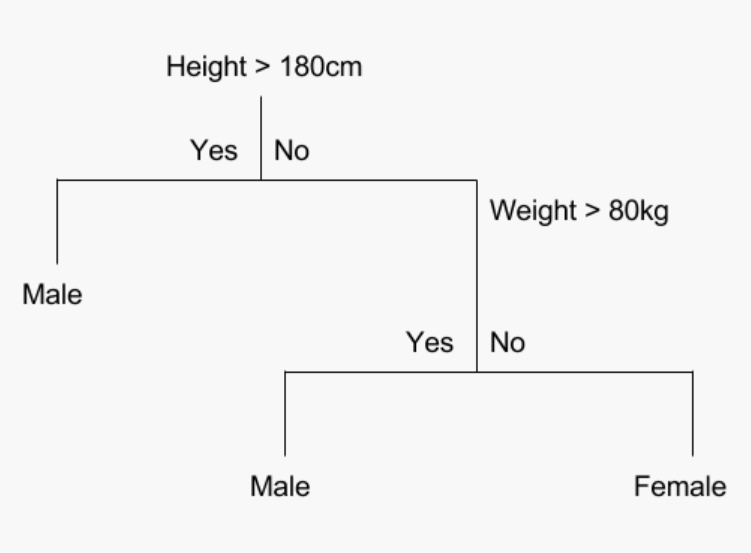
\includegraphics[width=3cm]{./figures/Binary_tree}
		\caption{Binary tree}
	\end{figure}

	\vspace{-0.5cm}

	\tiny Later in our presentation we will focus on  classification tree

\end{frame}
%%%%%%%%%%%%%%%%%%%%%%%%%%%%%%%%%%%%%%%%%%%%%%%%%%%%%%%%%%%%%%%%%%%%%%%%%%%%%%%%%%%%%%%%%%%%%%%%%%%

%%%%%%%%%%%%%%%%%%%%%%%%%%%%%%%%%%%%%%%%%%%%%%%%%%%%%%%%%%%%%%%%%%%%%%%%%%%%%%%%%%%%%%%%%%%%%%%%%%%
\begin{frame}
	\frametitle{Classification and Regression Trees}
		\framesubtitle{Problem}
	
		\vfill

		\begin{figure}
			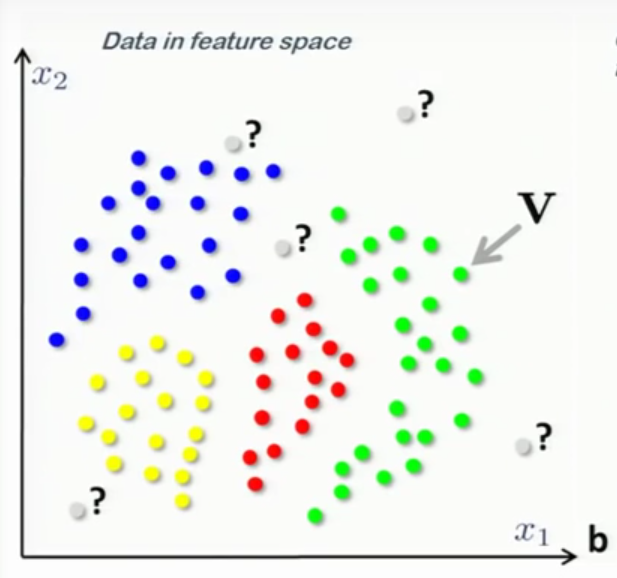
\includegraphics[width=6cm]{./figures/pastedImage0}
			\caption{Data in feature space}
		\end{figure}

		\vspace{-0.5cm}

\end{frame}
%%%%%%%%%%%%%%%%%%%%%%%%%%%%%%%%%%%%%%%%%%%%%%%%%%%%%%%%%%%%%%%%%%%%%%%%%%%%%%%%%%%%%%%%%%%%%%%%%%%

%%%%%%%%%%%%%%%%%%%%%%%%%%%%%%%%%%%%%%%%%%%%%%%%%%%%%%%%%%%%%%%%%%%%%%%%%%%%%%%%%%%%%%%%%%%%%%%%%%%
\begin{frame}
	\frametitle{Classification and Regression Trees}
		\framesubtitle{Solution}
	
		\begin{center}
		\begin{figure}[h]
		\begin{tabular}{ll}
		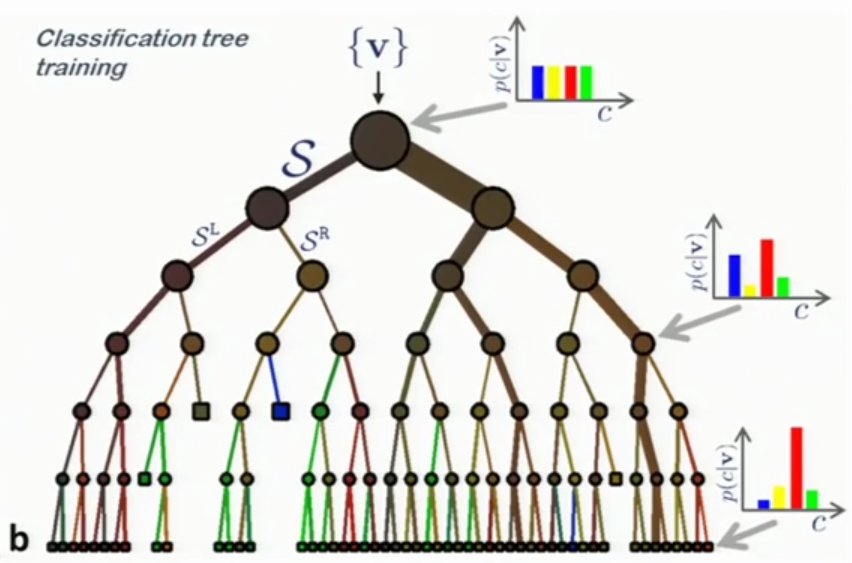
\includegraphics[width=7cm]{./figures/pastedImage1}
		&
		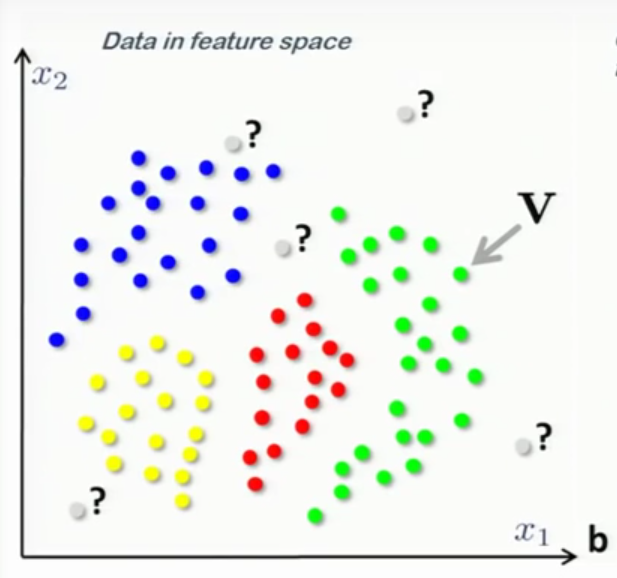
\includegraphics[width=3cm]{./figures/pastedImage0}
		\end{tabular}
		\caption{Classification tree training}
		\label{Fig:Race}
		\end{figure}
		\end{center}

\end{frame}
%%%%%%%%%%%%%%%%%%%%%%%%%%%%%%%%%%%%%%%%%%%%%%%%%%%%%%%%%%%%%%%%%%%%%%%%%%%%%%%%%%%%%%%%%%%%%%%%%%%

%%%%%%%%%%%%%%%%%%%%%%%%%%%%%%%%%%%%%%%%%%%%%%%%%%%%%%%%%%%%%%%%%%%%%%%%%%%%%%%%%%%%%%%%%%%%%%%%%%%
\begin{frame}
	\frametitle{Classification and Regression Trees}
		\framesubtitle{How to choose boundary? 
		Information gain}

		\begin{center}
		\begin{tabular}{m{4cm} m{6cm}}
		Below are listed four algorithms which allow to decide where to split:
		\begin{itemize}
		  \item[$\bullet$]  Gini index
		  \item[$\bullet$]  Chi-Square
		  \item[$\bullet$]  Information Gain
		  \item[$\bullet$]  Reduction in Variance
		\end{itemize}
		&
		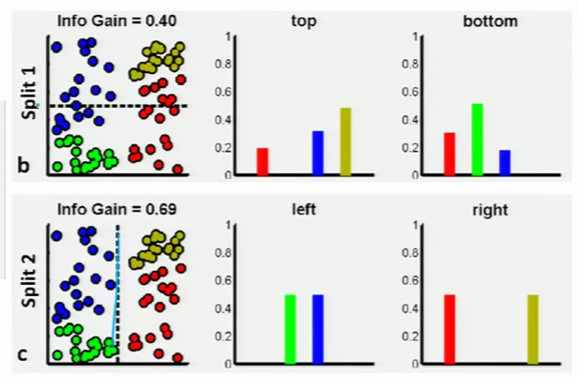
\includegraphics[width=6cm]{./figures/pastedImage2}\\
		&
		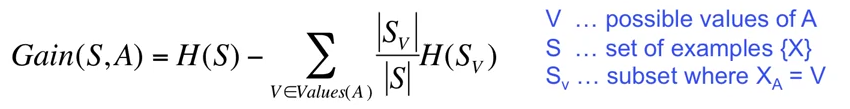
\includegraphics[width=6cm]{./figures/pastedImage3}
		\\
		\end{tabular}
		\end{center}
		
\end{frame}
%%%%%%%%%%%%%%%%%%%%%%%%%%%%%%%%%%%%%%%%%%%%%%%%%%%%%%%%%%%%%%%%%%%%%%%%%%%%%%%%%%%%%%%%%%%%%%%%%%%

\subsection{Building random tree} % Change, please!

%%%%%%%%%%%%%%%%%%%%%%%%%%%%%%%%%%%%%%%%%%%%%%%%%%%%%%%%%%%%%%%%%%%%%%%%%%%%%%%%%%%%%%%%%%%%%%%%%%%
\begin{frame}
	\frametitle{Classification and Regression Trees}
		\framesubtitle{Building a tree}
		\[
		X=
		\left[ {\begin{array}{ccccc}
		5 & 7 & 45 & 4 & 1\\
		3 & 7 & 8 & 7 & 2\\
		13 & 7 & 6 & 4 & 9
		\end{array} } \right]
		Y=
		\left[ {\begin{array}{ccccc}
		0 & 1 & 1 & 0 & 1
		\end{array} } \right]
		\] 
		It means 5 training examples, each defined by 3 features.
		\begin{center}
		\begin{tabular}{m{5cm} m{5cm}}
		1. Pick two features randomly.
		&
		2. Select possible split points, e.g. based on coordinates of points. \\
		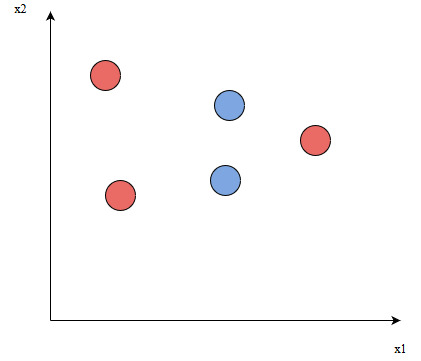
\includegraphics[width=4cm]{./figures/macierz1}
		&
		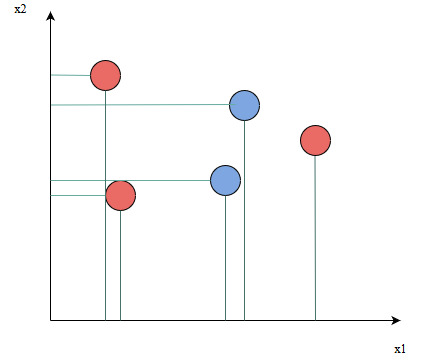
\includegraphics[width=4cm]{./figures/macierz2}
		\\
		\end{tabular}
		\end{center}
		
\end{frame}
%%%%%%%%%%%%%%%%%%%%%%%%%%%%%%%%%%%%%%%%%%%%%%%%%%%%%%%%%%%%%%%%%%%%%%%%%%%%%%%%%%%%%%%%%%%%%%%%%%%

%%%%%%%%%%%%%%%%%%%%%%%%%%%%%%%%%%%%%%%%%%%%%%%%%%%%%%%%%%%%%%%%%%%%%%%%%%%%%%%%%%%%%%%%%%%%%%%%%%%
\begin{frame}
	\frametitle{Classification and Regression Trees}
		\framesubtitle{Building a tree}

		\begin{center}
		\begin{tabular}{m{5cm} m{5cm}}
		3. Compute information gain and select the best split point
		&
		4. Splitted training examples .\\
		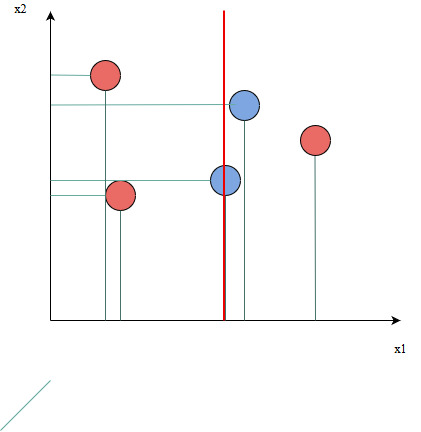
\includegraphics[width=5cm]{./figures/macierz4}
		&
		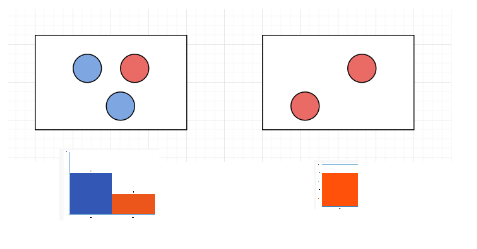
\includegraphics[width=5cm]{./figures/macierz5}
		\\
		\end{tabular}
		\end{center}
		
\end{frame}
%%%%%%%%%%%%%%%%%%%%%%%%%%%%%%%%%%%%%%%%%%%%%%%%%%%%%%%%%%%%%%%%%%%%%%%%%%%%%%%%%%%%%%%%%%%%%%%%%%%

%%%%%%%%%%%%%%%%%%%%%%%%%%%%%%%%%%%%%%%%%%%%%%%%%%%%%%%%%%%%%%%%%%%%%%%%%%%%%%%%%%%%%%%%%%%%%%%%%%%
\begin{frame}
	\frametitle{Classification and Regression Trees}
		\framesubtitle{Summary}

		
		\textbf{Advantages}
		\begin{center}
		\begin{itemize}
		  \item[$\bullet$] simple to understand, interpret, visualize
		  \item[$\bullet$] easily handle multi output problem
		  \item[$\bullet$] able to cope with nonlinear relations between parameters
		\end{itemize}
		
		\vfill
		
		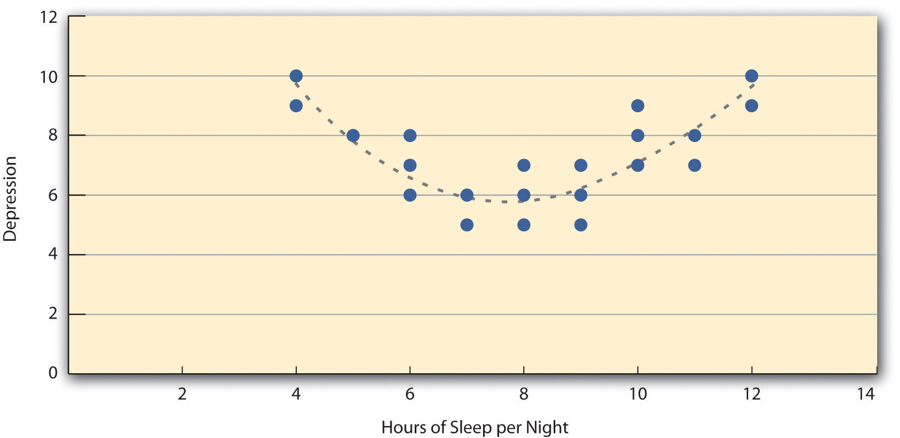
\includegraphics[width=7cm]{./figures/pros}
		\end{center}
		
\end{frame}
%%%%%%%%%%%%%%%%%%%%%%%%%%%%%%%%%%%%%%%%%%%%%%%%%%%%%%%%%%%%%%%%%%%%%%%%%%%%%%%%%%%%%%%%%%%%%%%%%%%

%%%%%%%%%%%%%%%%%%%%%%%%%%%%%%%%%%%%%%%%%%%%%%%%%%%%%%%%%%%%%%%%%%%%%%%%%%%%%%%%%%%%%%%%%%%%%%%%%%%
\begin{frame}
	\frametitle{Classification and Regression Trees}
		\framesubtitle{Summary}

		
		\textbf{Disadvantages}
		\begin{center}
		\begin{itemize}
		   \item[$\bullet$] overfitting, create complex trees do not generalize the data
		   \item[$\bullet$] simply too much data to load to the model 
		   \item[$\bullet$] big variance, decision tree can be unstable because small variation in data might result  in a completely different tree will be generated
		   \item[$\bullet$] can not guarantee to return globally optimal decision
		\end{itemize}
		
		\vfill
		
		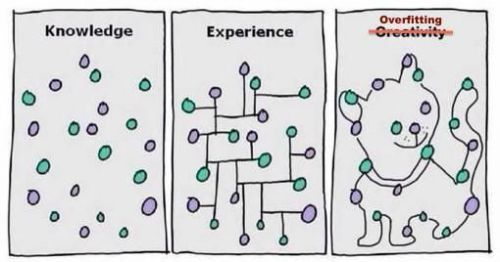
\includegraphics[width=5cm]{./figures/cons}
		\end{center}
		
\end{frame}
%%%%%%%%%%%%%%%%%%%%%%%%%%%%%%%%%%%%%%%%%%%%%%%%%%%%%%%%%%%%%%%%%%%%%%%%%%%%%%%%%%%%%%%%%%%%%%%%%%%

\subsection{Random forest} % Change, please!

%%%%%%%%%%%%%%%%%%%%%%%%%%%%%%%%%%%%%%%%%%%%%%%%%%%%%%%%%%%%%%%%%%%%%%%%%%%%%%%%%%%%%%%%%%%%%%%%%%%
\begin{frame}
	\frametitle{Random forest}
		\framesubtitle{Definition}

	\begin{block}{}
		Random forests or random decision forests are an ensemble learning method for classification, regression and other tasks, that operate by constructing a multitude of decision trees at training time and outputting the class that is the mode of the classes (classification) or mean prediction (regression) of the individual trees.
	\end{block}

	\vfill
	
	\begin{figure}
		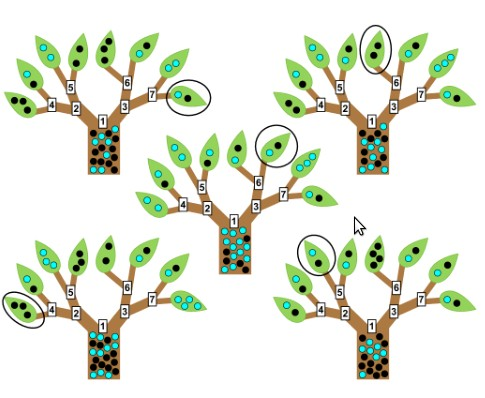
\includegraphics[width=4cm]{./figures/las}
	\end{figure}

\end{frame}
%%%%%%%%%%%%%%%%%%%%%%%%%%%%%%%%%%%%%%%%%%%%%%%%%%%%%%%%%%%%%%%%%%%%%%%%%%%%%%%%%%%%%%%%%%%%%%%%%%%

%%%%%%%%%%%%%%%%%%%%%%%%%%%%%%%%%%%%%%%%%%%%%%%%%%%%%%%%%%%%%%%%%%%%%%%%%%%%%%%%%%%%%%%%%%%%%%%%%%%
\begin{frame}
	\frametitle{Random forest}
		\framesubtitle{Definition}

		\begin{itemize}
		  \item[$\bullet$]  the term came from random decision forests that was first proposed by Tin Kam Ho of Bell Labs in 1995.
		  \item[$\bullet$] the method combines Breiman's "bagging" idea and the random selection of features.
		\end{itemize}
		
		\vfill
		
		For intuition:
		random forest builds multiple decision trees and merges them together to get a more accurate and stable prediction

		\vfill

		\tiny Later in our presentation we will focus on a classification aspect

\end{frame}
%%%%%%%%%%%%%%%%%%%%%%%%%%%%%%%%%%%%%%%%%%%%%%%%%%%%%%%%%%%%%%%%%%%%%%%%%%%%%%%%%%%%%%%%%%%%%%%%%%%

%%%%%%%%%%%%%%%%%%%%%%%%%%%%%%%%%%%%%%%%%%%%%%%%%%%%%%%%%%%%%%%%%%%%%%%%%%%%%%%%%%%%%%%%%%%%%%%%%%%
\begin{frame}
	\frametitle{Random forest}
		\framesubtitle{Algorithm}

	\vfill
	
	\begin{figure}
		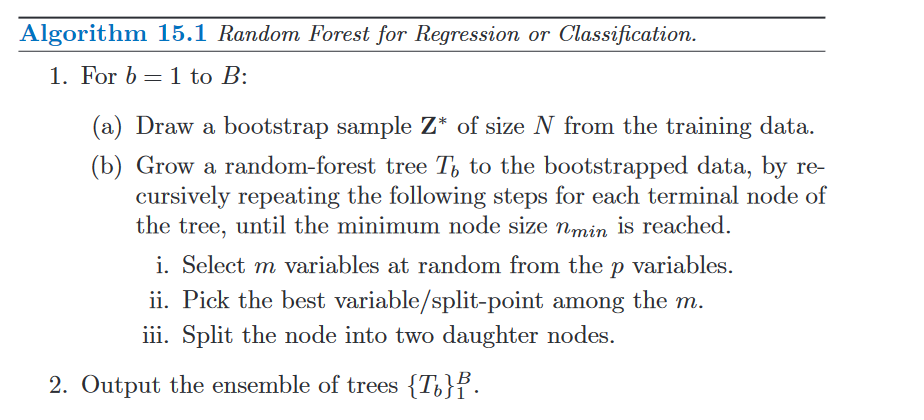
\includegraphics[width=12cm]{./figures/algorytm}
	\end{figure}

\end{frame}
%%%%%%%%%%%%%%%%%%%%%%%%%%%%%%%%%%%%%%%%%%%%%%%%%%%%%%%%%%%%%%%%%%%%%%%%%%%%%%%%%%%%%%%%%%%%%%%%%%%

%%%%%%%%%%%%%%%%%%%%%%%%%%%%%%%%%%%%%%%%%%%%%%%%%%%%%%%%%%%%%%%%%%%%%%%%%%%%%%%%%%%%%%%%%%%%%%%%%%%
\begin{frame}
	\frametitle{Random forest}
		\framesubtitle{Algorithm - bagging and boosting}
	
		\begin{center}
		\begin{figure}[h]
		\begin{tabular}{ll}
		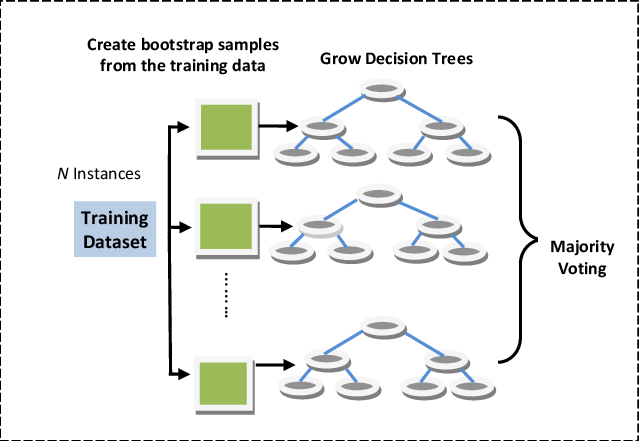
\includegraphics[width=6cm]{./figures/create}
		&
		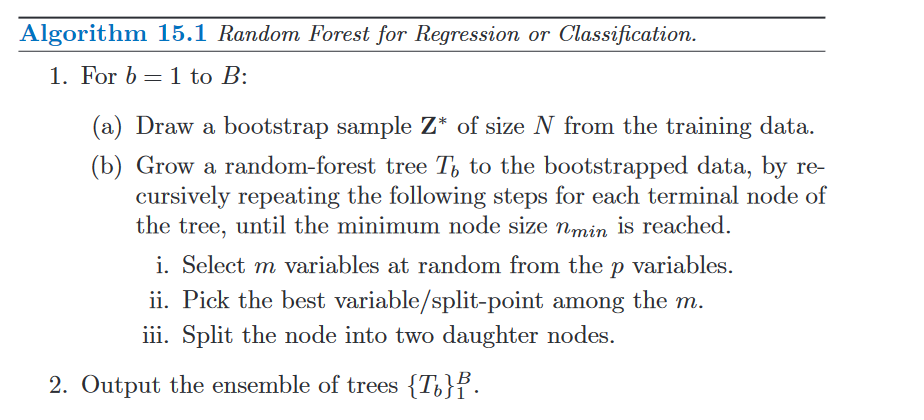
\includegraphics[width=5cm]{./figures/algorytm}
		\end{tabular}
		\end{figure}
		\end{center}

\end{frame}
%%%%%%%%%%%%%%%%%%%%%%%%%%%%%%%%%%%%%%%%%%%%%%%%%%%%%%%%%%%%%%%%%%%%%%%%%%%%%%%%%%%%%%%%%%%%%%%%%%%

%%%%%%%%%%%%%%%%%%%%%%%%%%%%%%%%%%%%%%%%%%%%%%%%%%%%%%%%%%%%%%%%%%%%%%%%%%%%%%%%%%%%%%%%%%%%%%%%%%%
\begin{frame}
	\frametitle{Random forest}
		\framesubtitle{Basic concept}

		\begin{center}
		\begin{tabular}{m{7cm} m{3cm}}
		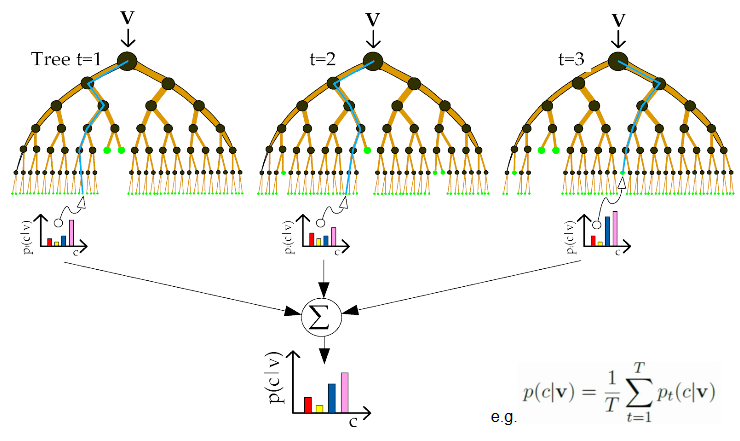
\includegraphics[width=7cm]{./figures/basic_concept}
		&
		Randomness in Random Forests:
		\begin{itemize}
		  \item 1) From data
		  \item 2) From splits in the features
		\end{itemize}
		\\
		\end{tabular}
		\end{center}
		
\end{frame}
%%%%%%%%%%%%%%%%%%%%%%%%%%%%%%%%%%%%%%%%%%%%%%%%%%%%%%%%%%%%%%%%%%%%%%%%%%%%%%%%%%%%%%%%%%%%%%%%%%%

\subsection{Random forest - examples} % Change, please!

%%%%%%%%%%%%%%%%%%%%%%%%%%%%%%%%%%%%%%%%%%%%%%%%%%%%%%%%%%%%%%%%%%%%%%%%%%%%%%%%%%%%%%%%%%%%%%%%%%%
\begin{frame}
	\frametitle{Random forest}
		\framesubtitle{Select number of trees - example}
	
		\begin{center}
		\begin{figure}[h]
		\begin{tabular}{cc}
		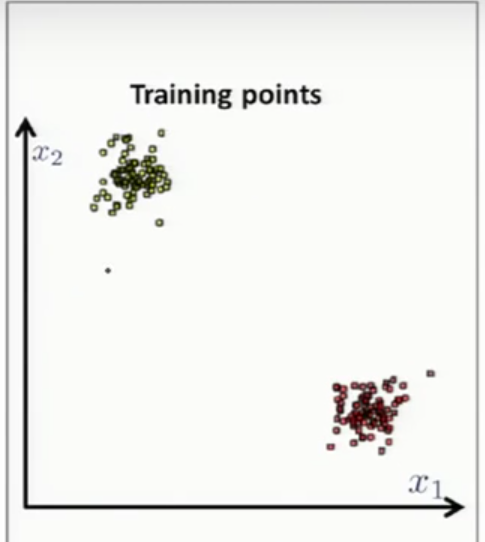
\includegraphics[width=3cm]{./figures/training_points}
		\\
		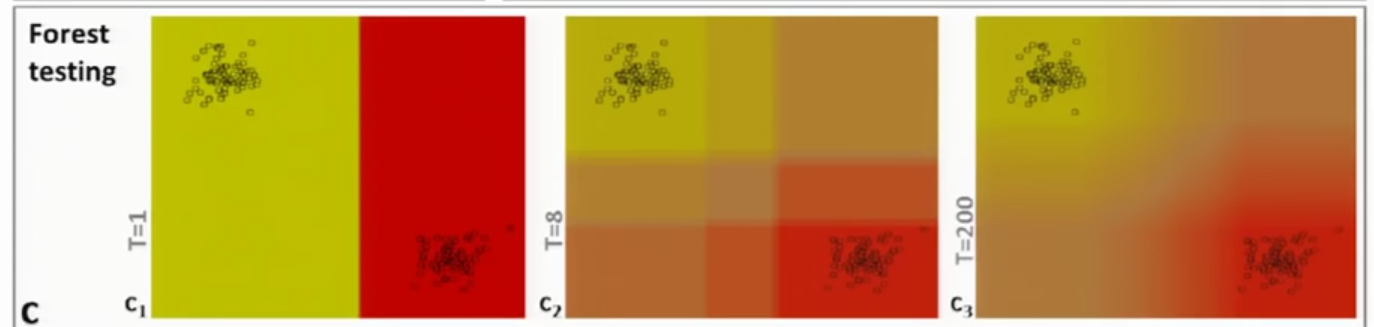
\includegraphics[width=10cm]{./figures/forest_testing}
		\end{tabular}
		\end{figure}
		\end{center}

\end{frame}
%%%%%%%%%%%%%%%%%%%%%%%%%%%%%%%%%%%%%%%%%%%%%%%%%%%%%%%%%%%%%%%%%%%%%%%%%%%%%%%%%%%%%%%%%%%%%%%%%%%

%%%%%%%%%%%%%%%%%%%%%%%%%%%%%%%%%%%%%%%%%%%%%%%%%%%%%%%%%%%%%%%%%%%%%%%%%%%%%%%%%%%%%%%%%%%%%%%%%%%
\begin{frame}
	\frametitle{Random forest}
		\framesubtitle{Many classes}
	
		\vfill
		
		\begin{figure}
			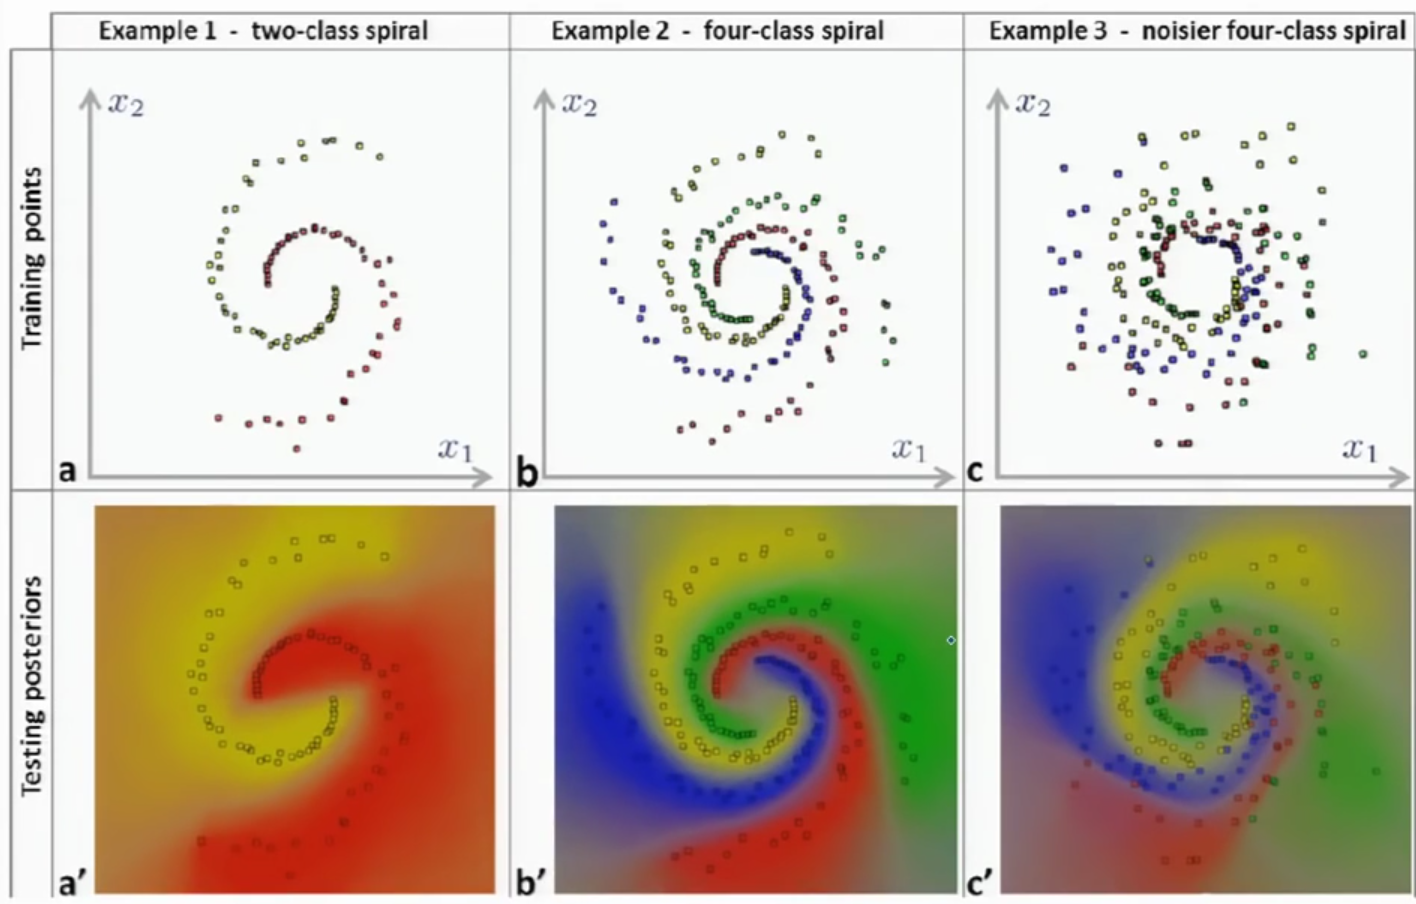
\includegraphics[width=10cm]{./figures/many_classes}
		\end{figure}

\end{frame}
%%%%%%%%%%%%%%%%%%%%%%%%%%%%%%%%%%%%%%%%%%%%%%%%%%%%%%%%%%%%%%%%%%%%%%%%%%%%%%%%%%%%%%%%%%%%%%%%%%%

%%%%%%%%%%%%%%%%%%%%%%%%%%%%%%%%%%%%%%%%%%%%%%%%%%%%%%%%%%%%%%%%%%%%%%%%%%%%%%%%%%%%%%%%%%%%%%%%%%%
\begin{frame}
	\frametitle{Random forest}
		\framesubtitle{Tree depth}
	
		\vfill
		
		\begin{figure}
			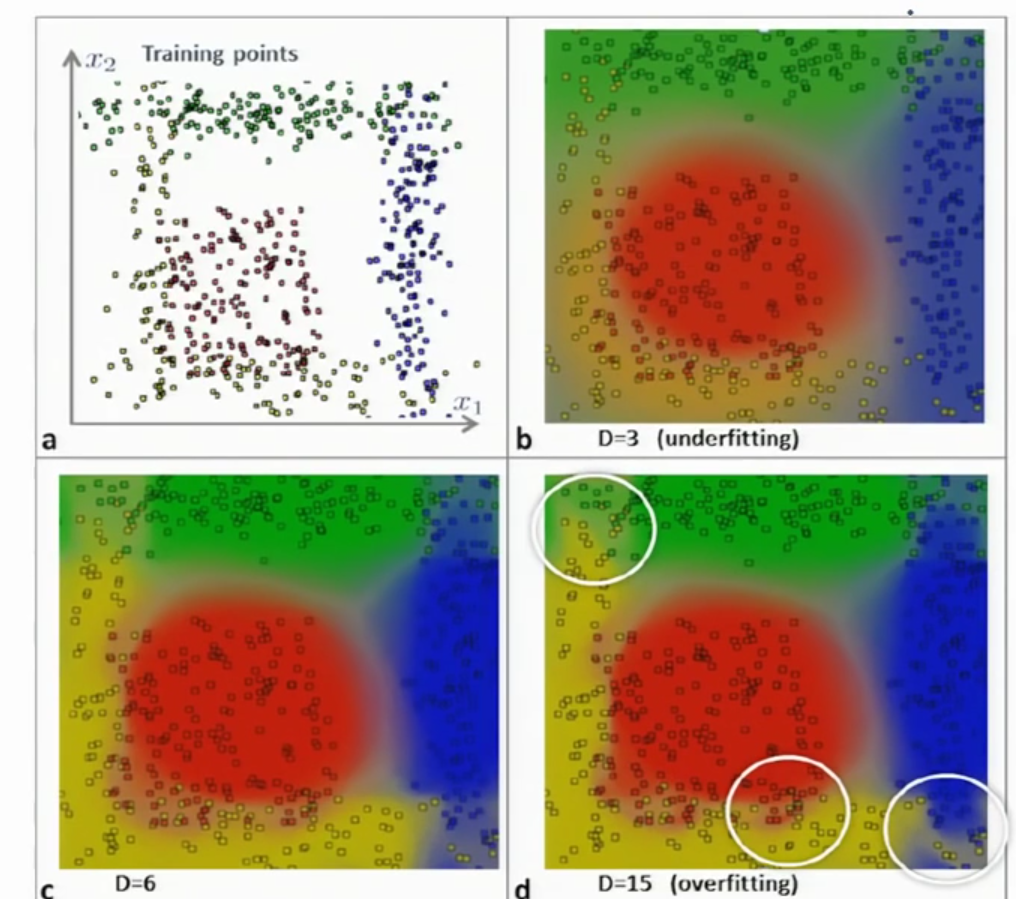
\includegraphics[width=7cm]{./figures/depth}
		\end{figure}

\end{frame}
%%%%%%%%%%%%%%%%%%%%%%%%%%%%%%%%%%%%%%%%%%%%%%%%%%%%%%%%%%%%%%%%%%%%%%%%%%%%%%%%%%%%%%%%%%%%%%%%%%%

%%%%%%%%%%%%%%%%%%%%%%%%%%%%%%%%%%%%%%%%%%%%%%%%%%%%%%%%%%%%%%%%%%%%%%%%%%%%%%%%%%%%%%%%%%%%%%%%%%%
\begin{frame}
	\frametitle{Random forest}
		\framesubtitle{Advantages}

		 \textbf{Advantages:}
		\begin{itemize}
		  \item[$\bullet$] the process of averaging or combining the results of different decision trees helps to overcome the problem of overfitting contrail to decision tree.
		  \item[$\bullet$] random forests also have less variance than a single decision tree. It means that it works correctly for a large range of data items than single decision trees.
		  \item[$\bullet$] random forests are extremely flexible and have very high accuracy.
		  \item[$\bullet$] they also do not require preparation of the input data. You do not have to scale the data.
		  \item[$\bullet$] it also maintains accuracy even when a large proportion of the data are missing.
		\end{itemize}

\end{frame}
%%%%%%%%%%%%%%%%%%%%%%%%%%%%%%%%%%%%%%%%%%%%%%%%%%%%%%%%%%%%%%%%%%%%%%%%%%%%%%%%%%%%%%%%%%%%%%%%%%%

%%%%%%%%%%%%%%%%%%%%%%%%%%%%%%%%%%%%%%%%%%%%%%%%%%%%%%%%%%%%%%%%%%%%%%%%%%%%%%%%%%%%%%%%%%%%%%%%%%%
\begin{frame}
	\frametitle{Random forest}
		\framesubtitle{Disadvantages}

		 \textbf{Disadvantages:}
		\begin{itemize}
		  \item[$\bullet$] overfitting is still observed 
		  \item[$\bullet$] need to choose the number of trees
		  \item[$\bullet$] they are not easily interpretable
		\end{itemize}

\end{frame}
%%%%%%%%%%%%%%%%%%%%%%%%%%%%%%%%%%%%%%%%%%%%%%%%%%%%%%%%%%%%%%%%%%%%%%%%%%%%%%%%%%%%%%%%%%%%%%%%%%%

\subsection{Demo} % Change, please!
\begin{frame}
\bigbreak
\bigbreak
\url{https://cs.stanford.edu/~karpathy/svmjs/demo/demoforest.html}\bigbreak
\url{http://www.r2d3.us/visual-intro-to-machine-learning-part-1/}\bigbreak
\url{https://arogozhnikov.github.io/2016/06/24/gradient_boosting_explained.html}\bigbreak
\url{https://arogozhnikov.github.io/2016/07/05/gradient_boosting_playground.html}
\end{frame}

%%%%%%%%%%%%%%%%%%%%%%%%%%%%%%%%%%%%%%%%%%%%%%%%%%%%%%%%%%%%%%%%%%%%%%%%%%%%%%%%%%%%%%%%%%%%%%%%%%%
\begin{frame}
	
	\begin{center}
		\Huge \textbf{Thank you for attention!}
	\end{center}

\end{frame}
%%%%%%%%%%%%%%%%%%%%%%%%%%%%%%%%%%%%%%%%%%%%%%%%%%%%%%%%%%%%%%%%%%%%%%%%%%%%%%%%%%%%%%%%%%%%%%%%%%% % Change, please!

%%%%%%%%%%%%%%%%%%%%%%%%%%%%%%%%%%%%%%%%%%%%%%%%%%%%%%%%%%%%%%%%%%%%%%%%%%%%%%%%%%%%%%%%%%%%%%%%%%%
%%%%%%%%%%%%%%%%%%%%%%%%%%%%%%%%%%%%%%%%%%%%%%%%%%%%%%%%%%%%%%%%%%%%%%%%%%%%%%%%%%%%%%%%%%%%%%%%%%%
%%%%%%%%%%%%%%%%%%%%%%%%%%%%%%%%%%%%%%%%%%%%%%%%%%%%%%%%%%%%%%%%%%%%%%%%%%%%%%%%%%%%%%%%%%%%%%%%%%%
%%%%%%%%%%%%%%%%%%%%%%%%%%%%%%%%%%%%%%%%%%%%%%%%%%%%%%%%%%%%%%%%%%%%%%%%%%%%%%%%%%%%%%%%%%%%%%%%%%%
%%%%%%%%%%%%%%%%%%%%%%%%%%%%%%%%%%%%%%%%%%%%%%%%%%%%%%%%%%%%%%%%%%%%%%%%%%%%%%%%%%%%%%%%%%%%%%%%%%%
%%%%%%%%%%%%%%%%%%%%%%%%%%%%%%%%%%%%%%%%%%%%%%%%%%%%%%%%%%%%%%%%%%%%%%%%%%%%%%%%%%%%%%%%%%%%%%%%%%%

%\bibliographystyle{plain}
%\nobibliography{bibliographyfile} % your bibliography file

\end{document}